%!TEX root = ../main.tex

\chapter{Hilbert Spaces}
\thispagestyle{empty}

We start by recalling what we have already done at Calculus \uppercase\expandafter{\romannumeral3} (Arioli) because more or less it is what we're going to discuss in this chapter.

\section{Calculus \uppercase\expandafter{\romannumeral3} recalls} % (fold)
\label{sec:calculus_3_recalls}

\subsection{Definizioni} % (fold)
\label{sub:definizioni}

\begin{defn}
[Prodotto scalare reale]
Sia $X$ uno spazio vettoriale. Si chiama prodotto scalare su $X$ una funzione $(\cdot,\cdot):X\times X\to\RR$ tale che per ogni $x,y,z\in X$ e per ogni $\lambda,\mu\in\RR$ si abbia
\begin{enumerate}
    \item [$\diamond$] $(x,x)\geq 0$ (positività)
    \item [$\diamond$] $(x,x)=0\ \Leftrightarrow\ x=0$ (annullamento)
    \item [$\diamond$] $(x,y)=(y,x)$ (simmetria)
    \item [$\diamond$] $(\mu x+\lambda y,z)=\mu(x,z)+\lambda(y,z)$ (linearità rispetto al primo argomento)
\end{enumerate}
\end{defn}
Sfruttando la proprietà di simmetria si può subito dire che la mappa $(\cdot,\cdot)$ è lineare anche rispetto al secondo argomento: si dice allora che il prodotto scalare è una \underline{forma bilineare simmetrica}.

Introduciamo ora la
\begin{defn}[Norma indotta dal prodotto scalare]
Sia $X$ uno spazio vettoriale e $(\cdot,\cdot)$ un prodotto scalare su $X$. Chiameremo norma indotta dal prodotto scalare la funzione definita da
\begin{equation*}
\Vert x\Vert =\sqrt{(x,x)} \qquad \forall x \in X
\end{equation*}
\end{defn}
Si può dimostrare che tale funzione è effetivamente una norma: le prime due proprietà sono banali, invece per la disuguaglianza triangolare
\begin{align*}
\Vert x+y \Vert ^2&=\Vert x \Vert^2+(x,y)+(y,x)+\Vert y \Vert^2= \\
&\overset{\underset{\text{SZ}}{}}{\leq} \Vert x \Vert^2+2\Vert x\Vert\,\Vert y\Vert +\Vert y \Vert^2= \\
&=\left(\Vert x\Vert+\Vert y\Vert\right)^2 \qquad \qquad \forall x,y\in X
\end{align*}

Il prodotto scalare e la norma sono quantità legate dal
\begin{thm}[di Schwarz]
Sia $X$ uno spazio vettoriale e $(\cdot,\cdot)$ un prodotto scalare su $X$. Allora per ogni $x,y\in X$ si ha
\begin{equation*}
|(x,y)|\leq \Vert x\Vert \cdot \Vert y \Vert\qquad (\text{SZ})
\end{equation*}
Il segno di uguaglianza vale se e solo se $x,y$ sono linearmente dipendenti.
\end{thm}

\begin{proof}
Prendiamo per comodità uno spazio vettoriale $X$ reale; siano dunque $t\in\RR$ e $x,y\in X$. Consideriamo il prodotto scalare
$$
(x-ty,x-ty)
$$
Per la proprietà di positività del prodotto scalare
$$
(x-ty,x-ty)\geq0
$$
Invece per la linearità rispetto al primo argomento e la simmetria
$$
(x-ty,x-ty)=\underbrace{\Vert x\Vert^2-2t(x,y)+t^2\Vert y\Vert^2}_{\text{polinomio di II grado in }t}
$$
Sappiamo che un polinomio del genere è $\geq 0$ se e solo se il suo discriminante è $\leq 0$, dunque si ottiene
$$
\frac{\Delta}{4}=(x,y)^2-\Vert x\Vert^2 \cdot \Vert y \Vert^2\leq 0
$$
Applicando la radice si ottiene proprio la disuguaglianza di Schwarz.
\end{proof}

Inoltre vale anche la
\begin{thm}[Identità del parallelogramma]
Sia $X$ uno spazio vettoriale e $(\cdot,\cdot)$ un prodotto scalare su $X$. Allora per ogni $x,y\in X$ si ha
\begin{equation*}
\left\|\frac{x+y}{2}\right\|^2+\left\|\frac{x-y}{2}\right\|^2=\frac{\Vert x\Vert^2 + \Vert y \Vert^2}{2}
\end{equation*}
\end{thm}

Siamo pronti per parlare di spazi di Hilbert.

\begin{defn}
[Spazio di Hilbert]
Uno spazio vettoriale dotato di prodotto scalare, che sia completo rispetto alla norma indotta dal prodotto scalare, è detto spazio di Hilbert.
\end{defn}
Quindi uno spazio di Hilbert non è altro che uno spazio vettoriale per il quale un prodotto scalare genera una norma che lo fa diventare uno spazio di Banach.

\textit{Esempio (dim finita).} 
$\RR^n$ è uno spazio di Hilbert rispetto al prodotto scalare
\begin{equation*}
(x,y)=\sum_{k=1}^n x_k\, y_k
\end{equation*}

\textit{Esempio (dim infinita).}
$\ell^{2}$ è uno spazio di Hilbert rispetto al prodotto scalare 
\begin{equation*}
(x,y)=\sum_{k=1}^\infty x_k\,y_k
\end{equation*}

\begin{marker}
Da qui capiamo chiaramente che lo spazio $\ell^2$ è la più naturale estensione dello spazio $\RR^n$. Infatti
\begin{align*}
\dim\RR^n=n \quad &\longrightarrow \quad \dim\ell^2=\infty \\
\text{vettori} \quad &\longrightarrow \quad \text{successioni} \\
\Vert x\Vert^2_{\RR^n}=\sum_{k=1}^n x_k^2 \quad &\longrightarrow \quad \Vert x\Vert^2_{\ell^2}=\sum_{k=1}^\infty x_k^2 \\
(x,y)_{\RR^n}=\sum_{k=1}^n x_k\, y_k \quad &\longrightarrow \quad (x,y)_{\ell^2}=\sum_{k=1}^\infty x_k\, y_k
\end{align*}
Detto terra terra: $\RR^\infty\approx\ell^2$.  
\end{marker}

% subsection definizioni (end)

\subsection{Proiezioni ortogonali in uno spazio di Hilbert} % (fold)
\label{sub:proiezioni_ortogonali_in_uno_spazio_di_hilbert}

\begin{defn}[Vettori ortogonali]
Sia $X$ spazio vettoriale. Due vettori $x,y\in X$ si dicono ortogonali se e solo se $(x,y)=0$.
\end{defn}

\begin{defn}
[Insieme convesso]
Sia $X$ spazio vettoriale. $C\subset X$ si dice convesso se $\forall x, y\in C$ e $\forall \lambda \in [0, 1]$ la combinazione convessa $\lambda x + (1 - \lambda) y\in C$.
\end{defn}

Dal punto di vista geometrico: $C$ è convesso se ``non ha rientranze'', ovvero il segmento congiungente $x$ e $y$ è sempre interno a $C$, qualsiasi punti $x,y$ si prendano:

\fg{0.4}{bonfa_14}

Parliamo ora di proiezioni (ortogonali). Dal punto di vista geometrico, la proiezione di un punto $x$ è

\fg{0.3}{bonfa_15}

cioè è una certa mappa $P:X\to X$ tale che $P^2=P$, ovvero se la proiezione di $x$ è $Px$, la proiezione di $Px$ è ancora $Px$.

Vale il

\begin{thm}
[Proiezione su un convesso chiuso]
Sia $\Hc$ uno spazio di Hilbert e $C\subset \Hc$ un convesso chiuso non vuoto. Allora per ogni $x\in \Hc$ esiste un'unica $y\in C$ tale che
\begin{equation*}
\Vert x - y \Vert =\inf_{z\in C} \Vert x-z \Vert
\end{equation*}
cioè che minimizza la distanza di $x$ da $C$; proprio per questo $y$ prende il nome di proiezione di $x$ su $C$ e viene indicata con $P_Cx$. 

Inoltre, se $\Hc$ è uno spazio reale, si ha
\begin{equation*}
(x-y,z-y)\leq 0\qquad \forall z \in C
\end{equation*}
cioè l'angolo $x\widehat{y}z$ è superiore all'angolo retto (al massimo uguale se $z=y$).
\end{thm}

Dal punto di vista geometrico

\fg{0.4}{bonfa_16}

\begin{defn}
[Spazio ortogonale]
Sia $\Hc$ di Hilbert e $M\subset \Hc$ un suo sottospazio vettoriale. Chiamiamo $M^{\perp}$ spazio ortogonale a $M$ il sottospazio vettoriale
\begin{equation*}
M^{\perp} = \{x\in \Hc\ :\ (x, y) = 0\ \ \forall y\in M\}
\end{equation*}
\end{defn}

Dal punto di vista geometrico

\fg{0.4}{bonfa_17}

Enunciamo ora il secondo teorema di proiezione:

\begin{thm}
[Proiezione su un sottospazio chiuso]
Sia $\Hc$ uno spazio di Hilbert e sia $M\subset \Hc$ un suo sottospazio vettoriale chiuso. Valgono i seguenti risultati:

\renewcommand{\theenumi}{\roman{enumi}}
\begin{enumerate}
    \item per ogni $ x\in \Hc$ esiste una proiezione $Px\in M$ tale che 
    $$
    \Vert x - Px \Vert =\inf_{z\in M} \Vert x-z \Vert
    $$
    \item detto $Qx=x-Px$ si ha che $Qx$ è la proiezione di $x$ su $M^{\perp}$ 
    \item vale Pitagora (generalizzato)
    $$
    \Vert x \Vert^{2} = \Vert Px \Vert^{2} + \Vert Qx \Vert^{2}
    $$
    \item le applicazioni $P: \Hc\rightarrow M$ e $Q: \Hc\rightarrow M^{\perp}$ sono lineari
\end{enumerate}
\end{thm}

Grazie a questo possiamo dire che esiste sempre un'unica decomposizione di $x$ in 
\begin{equation*}
\textcolor[rgb]{0.29, 0.56, 0.89}{x} = \textcolor[rgb]{0.82, 0.01, 0.11}{Px}+\textcolor[rgb]{0.49, 0.83, 0.13}{Qx}\qquad \text{con }Px\in M\text{ e }Qx\in M^\perp
\end{equation*}
Dal punto di vista geometrico ciò è ancora più chiaro:

\begin{figure}[htpb]
\centering
\tikzset{every picture/.style = {line width = 0.75pt}} %set default line width to 0.75pt

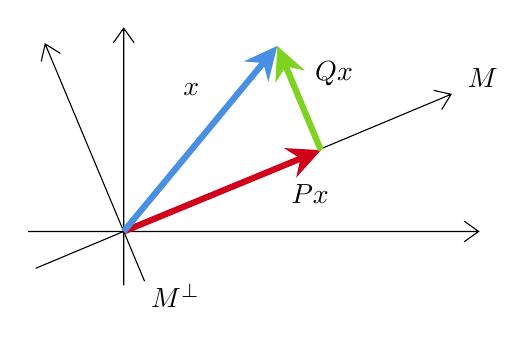
\begin{tikzpicture}[x = 0.75pt, y = 0.75pt, yscale = - 1, xscale = 1]
%uncomment if require: \path (0, 184); %set diagram left start at 0, and has height of 184

%Shape: Axis 2D [id: dp7134109691601231]
\draw (198, 127.91) - - (415, 127.91)(244, 30) - - (244, 153.91) (408, 122.91) - - (415, 127.91) - - (408, 132.91) (239, 37) - - (244, 30) - - (249, 37);
%Shape: Axis 2D [id: dp2976528104012621]
\draw (201.57, 145.68) - - (401.72, 61.83)(206.17, 37.6) - - (254.05, 151.89) (393.33, 59.93) - - (401.72, 61.83) - - (397.2, 69.15) (204.26, 45.99) - - (206.17, 37.6) - - (213.49, 42.13);
%Straight Lines [id: da6603280695196603]
\draw [color = {rgb, 255: red, 208; green, 2; blue, 27}, draw opacity = 1][line width = 2.25] (244, 127.91) - - (334.38, 90.66);
\draw [shift = {(339, 88.75)}, rotate = 517.6] [fill = {rgb, 255: red, 208; green, 2; blue, 27}, fill opacity = 1][line width = 0.08] [draw opacity = 0] (16.07, - 7.72) - - (0, 0) - - (16.07, 7.72) - - (10.67, 0) - - cycle;
%Straight Lines [id: da12421560052711267]
\draw [color = {rgb, 255: red, 74; green, 144; blue, 226}, draw opacity = 1][line width = 2.25] (244, 127.91) - - (314.81, 42.38);
\draw [shift = {(318, 38.53)}, rotate = 489.62] [fill = {rgb, 255: red, 74; green, 144; blue, 226}, fill opacity = 1][line width = 0.08] [draw opacity = 0] (16.07, - 7.72) - - (0, 0) - - (16.07, 7.72) - - (10.67, 0) - - cycle;
%Straight Lines [id: da9584665613249306]
\draw [color = {rgb, 255: red, 126; green, 211; blue, 33}, draw opacity = 1][line width = 2.25] (339, 88.75) - - (319.93, 43.15);
\draw [shift = {(318, 38.53)}, rotate = 427.31] [fill = {rgb, 255: red, 126; green, 211; blue, 33}, fill opacity = 1][line width = 0.08] [draw opacity = 0] (16.07, - 7.72) - - (0, 0) - - (16.07, 7.72) - - (10.67, 0) - - cycle;

% Text Node
\draw (408.5, 48.4) node [anchor = north west][inner sep = 0.75pt] {$M$};
% Text Node
\draw (256, 151.9) node [anchor = north west][inner sep = 0.75pt] {$M^{\perp}$};
% Text Node
\draw (271.5, 55.4) node [anchor = north west][inner sep = 0.75pt] {$x$};
% Text Node
\draw (335, 44.9) node [anchor = north west][inner sep = 0.75pt] {$Qx$};
% Text Node
\draw (323.5, 103.9) node [anchor = north west][inner sep = 0.75pt] {$Px$};
\end{tikzpicture}
\end{figure}
\FloatBarrier

\newpage

% subsection proiezioni_ortogonali_in_uno_spazio_di_hilbert (end)

\subsection{Basi hilbertiane e serie di Fourier generalizzata} % (fold)
\label{sub:basi_hilbertiane_e_serie_di_fourier_generalizzata}

\begin{defn}
Sia $\Hc$ uno spazio di Hilbert, $\dim \Hc=+\infty$. Sia $\{e_n\}_{n=1,2,\dots}\subset \Hc$ una successione di vettori di $\Hc$. Si dice che $\{e_n\}$ genera $\Hc$ se $\forall x\in \Hc$ e $\forall\Ec>0$ esiste una successione $\{\lambda_n\}_{n=1,\dots,N}$ tale che
$$
\left\|x-\sum_{n=1}^N\lambda_ne_n \right\|<\Ec
$$
\end{defn}
Ciò significa che è possibile generare uno spazio di dimensione \underline{infinita} con una combinazione lineare \underline{finita} di $\{e_n\}$, attraverso una \textit{tanto buona quanto si vuole} approssimazione.

\begin{rem}
Definendo le somme parziali della serie con $S_N=\sum_{n=1}^N\lambda_ne_n$ si può tradurre la relazione soprastante in 
$$
\lim_{N\to+\infty}S_N=x
$$
dove però è andato perduto il senso di convergenza in norma.
\end{rem}

\begin{defn}
[Base hilbertiana]
Sia $\Hc$ uno spazio di Hilbert, $\dim \Hc=+\infty$. Una successione di vettori $\{e_n\}_{n=1,2,\dots}\subset \Hc$ si dice base hilbertiana, o sistema ortonormale completo, se $\{e_n\}$ genera $\Hc$ ed è ortonormale, ovvero
$$
(e_n,e_m)=\delta_{nm}=
\begin{cases}
0 &m\neq n \\ 1 &m=n
\end{cases} \qquad \qquad \Vert e_n \Vert =1\ \ \forall n
$$
\end{defn}

Osserviamo due cose:
\begin{enumerate}
    \item Non essendo finita, una base hilbertiana non è una base nel senso dell'algebra lineare, ma è la cosa che più le si avvicina in dimensione infinita.
    \item La condizione $\Vert e_n \Vert =1$ è già implicita in $(e_n,e_m)=\delta_{nm}$.
\end{enumerate}

Se avessimo un generico spazio vettoriale $X$ finito potremmo scrivere
$$
x=\sum_{n=1}^Nc_ne_n
$$
e se la base fosse ortonormale potremmo addirittura calcolare i coefficienti della combinazione lineare tramite il prodotto scalare
$$
(x,e_n)=\left(\sum_{n=1}^Nc_ne_n,e_n\right)=\sum_{n=1}^Nc_n(e_n,e_n)=c_n
$$
Con una base hilbertiana vale un qualcosa di \textit{mooolto} simile:
\begin{thm}
\label{teoHNOsepa}
Sia $\Hc$ uno spazio di Hilbert, $\dim \Hc=+\infty$. Sia $\{e_n\}_{n=1,2,\dots}\subset \Hc$ una base hilbertiana. Allora un qualsiasi $x\in \Hc$ si scrive come \textbf{serie di Fourier generalizzata}
\begin{equation*}
\boxed{x = \sum^{+\infty}_{n = 1}(x, e_{n}) e_{n}}
\end{equation*}
I coefficienti $(x,e_n)=:\lambda_n$ della combinazione sono detti \textbf{coefficienti di Fourier} di $x$ rispetto $\{e_n\}$, e, come nel caso finito, sono dati da un prodotto scalare.
\end{thm}

Riprendendo il discorso di inizio pagina, abbiamo che la serie di Fourier generalizzata converge se e solo se
$$
\forall\Ec>0 \quad \exists N\in \NN \quad \text{t.c.}\quad \left\|x-\sum_{n=1}^N(x,e_n)e_n\right\|\leq \Ec
$$

% subsection basi_hilbertiane_e_serie_di_fourier_generalizzata (end)

\subsection{Spazi separabili} % (fold)
\label{sub:spazi_separabili}

Ora cercheremo di capire se, dato uno spazio di Hilbert generico, esiste una base hilbertiana. Per fare ciò riprendiamo le nozioni di numerabilità e di densità:

\begin{defn}[Insieme numerabile]
Si dice che l'insieme $A$ è numerabile se può essere messo in corrispondenza biunivoca con $\NN$.
\end{defn}
In pratica significa che possiamo \textit{mettere in fila} i suoi elementi:$A=\{a_1,a_2,a_3,\dots\}$.
\begin{defn}[Spazio denso]
Sia $X$ uno spazio normato e siano $A\subseteq B\subseteq X$. Si dice che $A$ è denso in $B$ se $\overline{A}=B$.
\end{defn}
In pratica significa che possiamo sempre costruire una successione in $V$ che approssima, nel senso della norma, lo spazio $\Hc$.
\begin{exa}
$\RR$ non è numerabile. $\QQ$ è denso in $\RR$.
\end{exa}

Siamo pronti:

\begin{defn}[Spazio separabile]
Uno spazio $\Hc$ di Hilbert si dice separabile se ammette un sottoinsieme denso e numerabile, ovvero se $\exists\,V\subset \Hc$ numerabile tale che $\overline{V}=\Hc$.
\end{defn}

\begin{thm}
Uno spazio $\Hc$ di Hilbert, $\dim \Hc=+\infty$, ammette una base hilbertiana se e solo se $\Hc$ è separabile.
\end{thm}

\begin{proof}\leavevmode
\begin{enumerate}
    \item [($\Rightarrow$)] Sia $\{e_n\}$ la base hilbertiana di $\Hc$. Allora la somma parziale $S_N$ è numerabile e approssima nel senso della norma $x\in \Hc$, per cui $\Hc$ è separabile.
    \item [($\Leftarrow$)] Sia $V\subset \Hc$ denso e numerabile. Allora è possibile costruire una base hilbertiana di $\Hc$ usando l'\textbf{algoritmo di ortogonalizzazione di Gram-Schmidt}:
    \begin{align*}
    V&=\left\{x_1,x_2,x_3,\dots \right\} \\
    e_1&=\frac{x_1}{\Vert x_1 \Vert} \\
    e_2&=\frac{x_2-(x_2,e_1)e_1}{\Vert x_2-(x_2,e_1)e_1 \Vert} \\
    e_3&=\frac{x_3-(x_3,e_1)e_1-(x_3,e_2)e_2}{\Vert x_3-(x_3,e_1)e_1-(x_3,e_2)e_2 \Vert} \\
    &\ \vdots
    \end{align*}
    Infatti i vettori $e_n$ sono ortogonali tra loro e hanno norma unitaria per costruzione; inoltre, essendo $V$ denso, generano $\Hc$.
\end{enumerate}
\end{proof}

% subsection spazi_separabili (end)

\subsection{Serie di Fourier generalizzata su spazi separabili} % (fold)
\label{sub:serie_di_fourier_generalizzata_su_spazi_separabili}

Ora riprendiamo a parlare di serie di Fourier generalizzate.

Grazie alla nozione di spazio di Hilbert separabile possiamo re-interpretare il teorema (\ref{teoHNOsepa}): è possibile sostituire all'ipotesi di esistenza della base hilbertiana $\{e_n\}$ la separabilità dello spazio di Hilbert considerato.

In ogni caso, una volta che sappiamo che esiste $\{e_n\}$ (che sia diretta conseguenza della separabilità oppure un'ipotesi) ha senso la seguente
$$
\Vert x\Vert^2=\sum_{n=1}^{+\infty} (x,e_n)^2 \qquad\qquad  \textbf{identità di Parseval}
$$
dove si ricorda che $(x,e_n):=\lambda_n$ sono i coefficienti di Fourier di $x$ rispetto la base $\{e_n\}$. Tale identità è banalmente verificabile:
\begin{align*}
\Vert x \Vert^2&=(x,x)=\left(\sum_{n=1}^{+\infty}(x,e_n)e_n,\sum_{k=1}^{+\infty}(x,e_k)e_k\right)=\\
&=\sum_{n=1}^{+\infty}\sum_{k=1}^{+\infty} (x,e_n)(x,e_k)\underbrace{(e_n,e_k)}_{\delta_{nk}}=\sum_{n=1}^{+\infty} (x,e_n)^2
\end{align*}

L'identità di Parseval permette di dire che la successione $\{\lambda_n\}$ dei coefficienti di Fourier è una successione a quadrato sommabile, ovvero $\{\lambda_n\}\subset \ell^2$ (se si parla di serie di Fourier elementare si ha $\{a_n\},\ \{b_n\}\in\ell^2$).

In realtà Parseval suggerisce qualcosa in più: è possibile definire un'applicazione $L:\Hc\to\ell^2$ che associa ad ogni $x\in \Hc$ la successione $\lambda=\{\lambda_n\}=\{(x,e_n)\}\subset\ell^2$ dei suoi coefficienti di Fourier rispetto alla base $\{e_n\}$; tale applicazione è ovviamente \underline{lineare}
$$
(ax+by,e_n)=a(x,e_n)+b(y,e_n)
$$
\underline{isometrica} (stessa metrica su dominio e codominio)
$$
\Vert Lx \Vert_{\ell^2}=\Vert \lambda \Vert_{\ell^2}=\left(\sum_{n=1}^{+\infty}\lambda_n^2\right)^{1/2} =\Vert x \Vert_H
$$
e di conseguenza anche \underline{iniettiva} e \underline{continua}. 

Tutto questo, in \textit{matematichese}, si traduce in
\begin{thm}
Sia $\Hc$ uno spazio di Hilbert separabile di dimensione infinita. Allora $\Hc$ è isomorfo e isometrico allo spazio $\ell^2$, cioè esiste un \textbf{isomorfismo isometrico}
\begin{align*}
L:\Hc&\to\ell^2 \\
x&\mapsto Lx=\{(x,e_n)\}
\end{align*}
\end{thm} 

\begin{proof}
Per dimostrare l'asserto dobbiamo dimostrare che $\Hc$ e $\ell^2$ sono isometrici, cioè sono dotati della stessa metrica, e isomorfi, cioè $L$ è una mappa lineare continua e biunivoca.

Ma che i due spazi sono isometrici
\begin{equation*}
\Vert Lx \Vert_{\ell^2}=\Vert x \Vert_\Hc \qquad \forall x\in \Hc
\end{equation*}
e che $L$ è lineare continua e iniettiva l'avevamo già dedotto dall'identità di Parseval.

Dunque l'unica cosa che veramente viene aggiunta da questo teorema è la \underline{suriettività} di $L$: per dimostrare quest'ultima bisogna prendere $a=(a_1,a_2,\dots)\in\ell^2$ e verificare che $Lx=a$. 

Consideriamo allora la somma parziale
$$
x_n:=\sum_{k=1}^na_ke_k
$$
Sappiamo due cose: che $\sum_{k=1}^\infty a_k^2$ converge (per definizione di $\ell^2$) e che gli $e_k$ sono ortonormali (per definizione di base hilbertiana). Da ciò si deduce che per ogni $\Ec>0$ esiste $N\in \NN$ tale che per ogni $n>m>N$
$$
\Vert x_n-x_m\Vert_\Hc^2=\left\|\sum_{k=m+1}^n a_ke_k\right\|^2=\sum_{k=m+1}^n a_k^2<\Ec
$$
Pertanto la successione $\{x_n\}$ è di Cauchy in $\Hc$ ed essendo quest'ultimo completo esiste $x\in \Hc$ tale che $x_n\to x$. Si verifica immediatamente che i coefficienti di Fourier di $x$ coincidono con gli $a_k$ e quindi $Lx=a$: $L$ è suriettiva.
\end{proof}

\begin{rem}
Tale teorema è l'estensione infinito-dimensionale al teorema che mette in corrispondenza un insieme qualsiasi di dimensione $n$ a $\RR^n$.
\end{rem}

% subsection serie_di_fourier_generalizzata_su_spazi_separabili (end)


% section calculus_3_recalls (end)

\section{Definitions and Elementary Properties} % (fold)
\label{sec:definitions_and_elementary_properties}

\begin{defn}
$\Hc$ (real) vector space. Then, a function $p:\Hc\times \Hc\to\RR$ is a \textbf{scalar product} or \textbf{inner product} if:
\begin{enumerate}
\item positivity holds:
\begin{equation*}
    p(x,x)\geq 0,\qquad\qquad p(x,x)=0\quad \Longleftrightarrow\quad x=0
\end{equation*}

\item simmetry holds:
\begin{equation*}
    p(x,y)=p(y,x)
\end{equation*}

\item bilinearity holds:
\begin{equation*}
    p(\alpha x +\beta y, z)=\alpha p(x,z)+ \beta p(y,z)
\end{equation*}
\end{enumerate}
$\forall x,y,z\in \Hc,\ \forall \alpha,\beta\in\RR$. 
\end{defn}

\underline{Notation}: one can identify the scalar product with
\begin{equation*}
    p(x,y)=\sca{x,y}=(x,y)=x\cdot y
\end{equation*}
but we use the second one.

\begin{defn}
$\left( \Hc,\sca{\cdot,\cdot} \right)$ is a \textbf{pre-Hilbertian space} or \textbf{inner product space}.
\end{defn}

\begin{proposition}
$\left( H,\sca{\cdot,\cdot} \right)$ pre-Hilbert. Then:
\begin{enumerate}
\item the \textbf{Cauchy-Schwarz Inequality} holds:
\begin{equation*}
    \abs{\sca{x,y}}\leq \sqrt{\sca{x,x}}\cdot\sqrt{\sca{y,y}}\qquad \forall x,y\in \Hc
\end{equation*}

\item define the \textbf{induced norm} (by the scalar product) $\norm{x}=\sqrt{\sca{x,x}}$, then
\begin{equation*}
    \left( \Hc,\norm{\cdot} \right)\text{ is a normed space}
\end{equation*}

\item the \textbf{Parallelogram Identity} holds: $\norm{x+y}^2+\norm{x-y}^2=2\norm{x}^2+2\norm{y}^2$ or
\begin{equation*}
\norm{\frac{x+y}{2}}^2+\norm{\frac{x-y}{2}}^2=\frac{\norm{x}^2+\norm{y}^2}{2} \qquad\forall x,y\in \Hc
\end{equation*}
\end{enumerate}
\end{proposition}

\begin{proof}\leavevmode
\begin{enumerate}
\item same as in $\RR^N$
\item exercise (to check the triangle inequality use Cauchy-Schwarz)
\item $\sca{x\pm y,x\pm y}=\sca{x,x}\pm\sca{x,y}+\sca{y,y}$
\end{enumerate}
\end{proof}

\begin{marker}
The chain is the following:

\begin{equation*}
{\renewcommand*{\arraystretch}{1.5}
\begin{array}{cl}
 \left(X, \sca{\cdot,\cdot} \right) & \text{inner product space} \\
\big\downarrow {\scriptstyle \text{induces} } & \\
\left(X, \norm{\cdot} \right) & \text{normed space, with } \norm{x}=\sqrt{\sca{x,x}} \\
\big\downarrow {\scriptstyle \text{induces} } & \\
\left(X, \sca{\cdot,\cdot} \right) & \text{metric space, with } d(x,y)=\norm{x-y} \\
\big\downarrow {\scriptstyle \text{induces} } & \\
\text{topology, convergence, etc.}
\end{array}}
\end{equation*}
\end{marker}

\begin{defn}
$\left( \Hc,\sca{\cdot,\cdot} \right)$ inner product space is a \textbf{Hilbert space} if it is complete with respect to the induced norm (i.e. $\left( \Hc,\norm{\cdot} \right)$ is Banach).
\end{defn}

\textit{Example.}
$\RR^N$ equipped with the euclidian scalar product is Hilbert.

\textit{Example.}
Let $\left( X,\Mdu,\mu \right)$ be a complete measure space, then $L^2\left( X,\Mdu,\mu \right)$ equipped with
\begin{equation*}
    \sca{u,v}_{L^2}=\int_X uv\demu
\end{equation*}
is a Hilbert space, and the induced norm is the one we're expecting:
\begin{equation*}
    \norm{u}=\left( \int_X u^2\demu \right)^{1/2}=\norm{u}_2
\end{equation*}

In particular, $\ell^2$ equipped with
\begin{equation*}
\sca{x,y}=\sum_{i\in\NN}x_i y_i
\end{equation*}
is Hilbert too.

\textit{Example.}
$\left( \Cc\left( [a,b] \right),\sca{\cdot,\cdot}_{L^2} \right)$ is pre-Hilbert but not Hilbert.

\textit{Example.}
The Sobolev space $\Hc^1$ (as everyone has seen in EDP (if you didn't, just re-enroll the bachelor), it's the space of $L^2$ functions that have weak derivatives in $L^2$) is another example of a Hilbert space.

\bigskip
\bigskip

We know that $X$ Hilbert $\Longrightarrow$ $X$ Banach, but ... \\
\boxed{Q} It is possibile to check the $\Longleftarrow$, i.e. to check if given a norm there exists a scalar product inducing that?

\smallskip

The answer is yes, thanks to the parallelogram identity:

\begin{proposition}[Fréchet – von Neumann – Jordan)]
$\left( X,\norm{\cdot} \right)$ Banach. Then, it is also Hilbert iff $\norm{\cdot}$ satisfies the parallelogram identity. Hence, the scalar product is defined as
\begin{equation*}
    \sca{x,y}:=\frac{1}{4}\left( \norm{x+y}^2-\norm{x-y}^2 \right)
\end{equation*}
\end{proposition}

As a consequence, we can check that a space does not have a scalar product. For example:
\begin{itemize}
    \item $\left( L^p,\norm{\cdot}_p \right)$ is not Hilbert for $p\neq 2$
    \item $\Big( \Cc\left( [a,b] \right),\norm{\cdot}_\infty \Big)$ is not Hilbert
\end{itemize}

% section definitions_and_elementary_properties (end)

\section{Projections onto a Closed Convex Set} % (fold)
\label{sec:projections_onto_a_closed_convex_set}

We start with some recalls. Let $\Hc$ Hilbert space.
\begin{enumerate}[(i)]
\item $S\subset \Hc$ is convex if
\begin{equation*}
    x,y\in S,\ t\in[0,1]\quad\Longrightarrow\quad tx+(1-t)y \in S
\end{equation*}

\item $x,y\in \Hc$ are orthogonal, and we write $x\perp y$, iff $\sca{x,y}=0$

\item given $V\subset \Hc$, the \textbf{orthogonal complement} of $V$ is
\begin{equation*}
V^\perp :=\left\{ w\in \Hc\,:\,\sca{w,v}=0\quad\forall v\in V \right\}
\end{equation*}

\item $S\subset \Hc$, $x\in \Hc$, then
\begin{equation*}
\text{dist}(x,S):=\inf_{v\in S} \norm{x-v}
\end{equation*}
\end{enumerate}

\newpage

\begin{thm}[Projection theorem on closed convex sets]$\\$
$\Hc$ Hilbert, $x\in \Hc$, $S\subset \Hc$ non-empty closed convex set. Then:
\begin{equation}
\label{proj_1}
\exists !\,h\in S\quad \text{s.t.}\quad \norm{x-h}=\min_{v\in S}\norm{x-v}=\text{dist}(x,S)
\end{equation}

Moreover, $h$ is characterized\footnote{$\ h$ satisfies (\ref{proj_1}) iff $h$ satisfies (\ref{proj_2})} by the \emph{variational inequality}
\begin{equation}
\label{proj_2}
\sca{x-h,v-h}\leq 0\qquad\forall v\in S
\end{equation}
\end{thm}

\underline{Notation}: the above element $h$ is called the projection of $x$ onto $S$ and it is denoted by
\begin{equation*}
h=P_Sx=\text{proj}_S x
\end{equation*}

\begin{marker}
Relation (\ref{proj_1}) says that the infimum is actually a minimum. 

Inequality (\ref{proj_2}) says that the scalar product of the vector $\underline{hx}$ with any vector $\underline{hv}$ is $\leq 0$, i.e., the angle determined by these two vectors is $\geq \pi/2$ (see Figure \ref{proj_fig}).
\end{marker}

\begin{figure}[H]
\begin{center}
  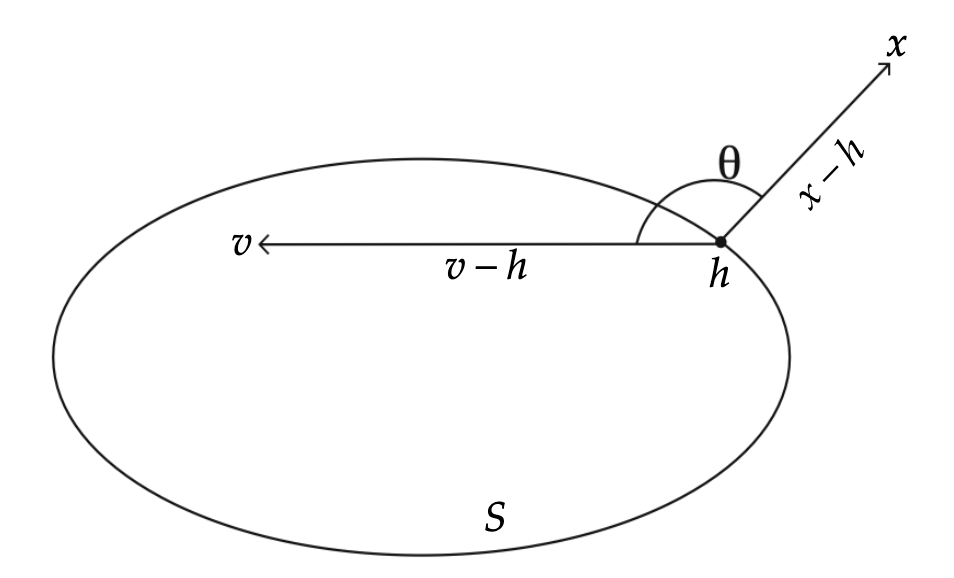
\includegraphics[width=8cm]{images/bonfa_1150}
\end{center}
\caption{}
\label{proj_fig}
\end{figure}

\begin{proof}[forgive me for excessive repetitions] $\\$
We need to prove existence and uniqueness of $h\in S$ which satisfies (\ref{proj_1}), and then (\ref{proj_1}) $\Longleftrightarrow$ (\ref{proj_2}).

\begin{enumerate}[(a)]
\item \emph{Existence.} How do we prove that there exists a minimizer of something? We take a minimizing sequence and we try to see if it converges; if it converges, then its limit is the candidate minimum.

Let's call
\begin{equation*}
    d:=\inf_{v\in S}\norm{x-v}
\end{equation*}
so $d$ is a non-negative number which satisfies
\begin{equation*}
\qquad\qquad\qquad\qquad\qquad\qquad\qquad\qquad d \leq \norm{x-s}\qquad \forall s\in S \qquad\qquad\qquad\qquad \qquad\qquad\qquad\qquad \circledast
\end{equation*}

We take a minimizing sequence:
\begin{equation*}
\exists \left\{ v_n \right\}_{n\in\NN}\subset S\quad\text{s.t.}\quad d\leq \norm{x-v_n}\leq d+\frac{1}{n} 
\end{equation*}

(we have only applied the definition of infimum, as we have done several times during the course)

We are going to show that $\left\{ v_n \right\}_n$ is a Cauchy sequence (i.e., $\norm{v_n-v_m}\to 0$ as $n,m\to\infty$) and, since we have completness of the space, it implies that $\left\{ v_n \right\}$ converges. In order to obtain it, we apply the parallelogram identity to
\begin{equation*}
    x-v_n\qquad\text{and}\qquad x-v_m
\end{equation*}

We have:
\begin{gather*}
\norm{(x-v_n)+(x-v_m)}^2+\norm{(x-v_n)-(x-v_m)}^2=2\norm{x-v_n}^2+2\norm{x-v_m}^2 \\ 
\norm{2x-v_n-v_m}^2+\underbracket[0.2pt]{\norm{v_m-v_n}^2}_{\text{what we want}}=2\norm{x-v_n}^2+2\norm{x-v_m}^2 \\ 
\norm{v_m-v_n}^2=2\norm{x-v_n}^2+2\norm{x-v_m}^2 -4\norm{x- \frac{v_n+v_m}{2} }^2
\end{gather*}

Since $S$ is convex $\dfrac{v_n+v_m}{2}\in S$, thus thanks to $\circledast$ we know that
\begin{equation*}
\norm{x- \frac{v_n+v_m}{2} } \geq d
\end{equation*}

Finally:
\begin{equation*}
0\leq \norm{v_m-v_n}^2 \leq 2\underbracket[0.2pt]{\norm{x-v_n}^2}_{\xrightarrow[]{n\to\infty} d^2}+2\underbracket[0.2pt]{\norm{x-v_m}^2}_{\xrightarrow[]{m\to\infty} d^2} -4d^2 \xrightarrow[]{n,m\to\infty} 0
\end{equation*}

This implies that $\left\{ v_n \right\}$ is a Cauchy sequence, and since $\Hc$ is Hilbert (in particular, it is complete), $\left\{ v_n \right\}$ is converging:
\begin{equation*}
    \exists h\in \Hc\quad\text{s.t.}\quad v_n\to h\quad\text{in }\Hc
\end{equation*}

By now, we used the completness of $\Hc$ and we found a candidate minimum in $\Hc$, but this is not what we want. Indeed, the situation is shown in Figure \ref{proj_fig2}.

We use that $S$ is closed, i.e.
\begin{equation*}
    \begin{cases}
        \left\{ v_n \right\}_n\subset S \\
        v_n\to h\quad\text{in }H
    \end{cases}
    \qquad\Longrightarrow\qquad h\in S
\end{equation*}

So we have found the candidate minimum in the right place.

Thanks to continuity of $\norm{\cdot}$ (in normed spaces the norm is continuous because of the tr. inequality), we can pass to the limit and obtain
\begin{gather*}
d\leq \norm{x-v_n}\leq d+\frac{1}{n} \\
\Big\downarrow n\to\infty \\
d\leq \norm{x-h}\leq d
\end{gather*}

$\Longrightarrow \norm{x-h}=d=\text{dist}(x,S)$

\item \emph{Uniqueness.} By contradiction, we assume $\exists\,h_1,h_2$, $h_1\neq h_2$, s.t. $\norm{x-h_1}=\norm{x-h_2}=d$. We apply the parallelogram identity to $x-h_1$ and $x-h_2$:
\begin{gather*}
\underbracket[0.2pt]{\norm{x-h_1+x-h_2}^2}_{\geq 4d^2}+\underbracket[0.2pt]{\norm{x-h_1-(x-h_2)}^2}_{=\norm{h_2-h_1}^2}=2\underbracket[0.2pt]{\norm{x-h_1}^2}_{= d^2}+2\underbracket[0.2pt]{\norm{x-h_2}^2}_{= d^2} \\
\Longrightarrow\quad 0\leq \norm{h_2-h_1}^2\leq 0
\end{gather*}
and by positivity of the norm we obtain $h_1=h_2$, which contradict the assumption.

\item \emph{Equivalence of (\ref{proj_1}) and (\ref{proj_2}).} We know $h\in S$, take any $v\in S$, $t\in[0,1]$, thus
\begin{equation*}
    (1-t)h+tv \in S
\end{equation*}

and, thanks to $\circledast$,
\begin{gather*}
\norm{x-\left[ (1-t)h+tv \right]}^2\geq \norm{x-h}^2 \\
\norm{(x-h)-t(v-h)}^2 \geq \norm{x-h}^2 \\
\cancel{\norm{x-h}^2}-2\cancel{t}\sca{x-h,v-h}+t^{\cancel{2}}\norm{v-h}^2\geq \cancel{\norm{x-h}^2} \qquad (t\neq 0) \\
\qquad \sca{x-h,v-h}\leq \frac{t}{2}\norm{v-h}^2\qquad\ \forall 0<t\leq 1
\end{gather*}

Taking the limit as $t\to 0^+$ we get (\ref{proj_2}).

Conversely, assume that $h$ satisifes (\ref{proj_2}). We have to prove that 
\begin{equation*}
\norm{x-h}^2\leq \norm{x-v}^2\qquad\text{for any }v\in S
\end{equation*}

so let's study 
\begin{align*}
\norm{x-h}^2-\norm{x-v}^2 &= \norm{x-h}^2-\norm{x-\textcolor{red}{h}+\textcolor{red}{h}-v}^2 = \\
&= \norm{x-h}^2-\norm{(x-h)-(v-h)}^2 = \\
&= \cancel{\norm{x-h}^2}- \left[ \cancel{\norm{x-h}^2} -2 \sca{x-h,v-h} + \norm{v-h}^2 \right] = \\
&=\underbracket[0.2pt]{2 \sca{x-h,v-h}}_{\leq 0}-\underbracket[0.2pt]{\norm{v-h}^2}_{\geq 0} \leq 0
\end{align*}

which concludes the proof.
\end{enumerate}
\end{proof}

\begin{figure}[H]
\begin{center}
  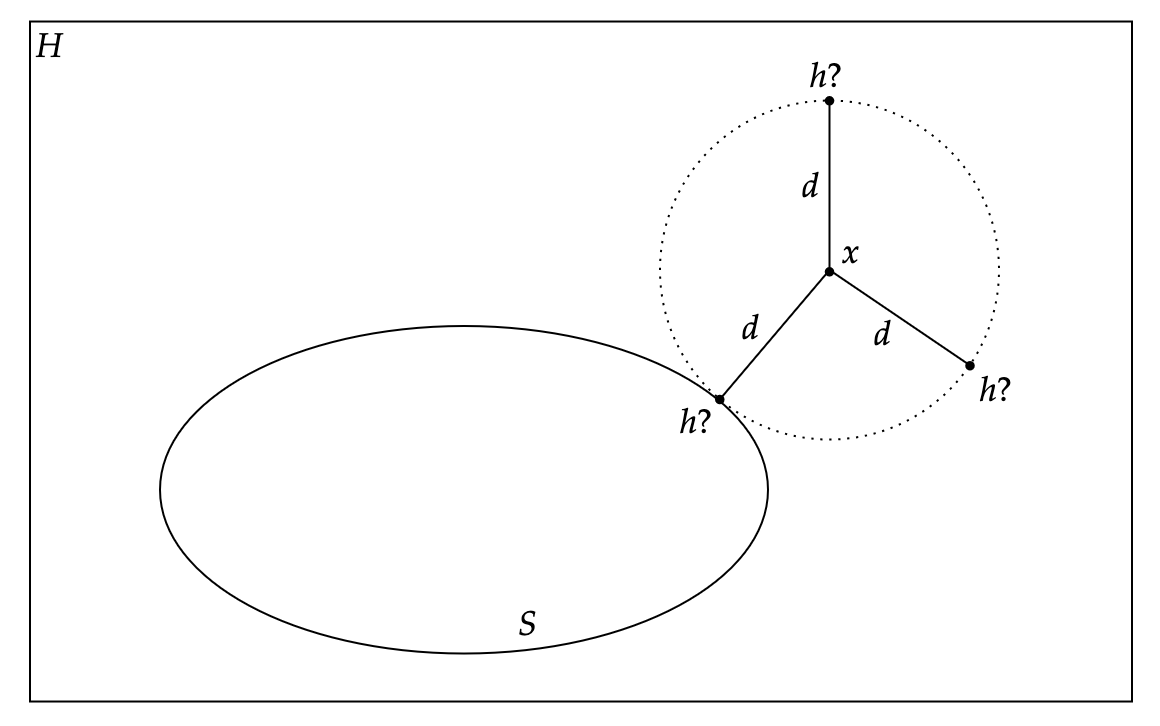
\includegraphics[width=9cm]{images/bonfa_0933.png}
\end{center}
\caption{}
\label{proj_fig2}
\end{figure}

What we really need is the following \emph{very important} particular case: when $S$ is a closed vector subspace, since it is convex too, we can apply the previous theorem and obtain:

\begin{thm}[Projection theorem for closed subspaces]$\\$
$\Hc$ Hilbert, $x\in \Hc$, $V\subset \Hc$ closed subspace. Then:
\begin{equation*}
\exists !\,h\left( =P_Vx \right)\in V\quad \text{s.t.}\quad \norm{x-h}=\min_{v\in V}\norm{x-v}
\end{equation*}

Moreover, $h$ is characterized by the \emph{variational equality}
\begin{equation}
\label{proj_3}
\sca{x-h,v}=0\qquad\forall v\in V
\end{equation}
\end{thm}

This version is actually the reason why we call $h$ the orthogonal projection.

\newpage


\textbf{Mnemonic rule.} In the particular case of closed subspaces "you have \emph{only} the line"

\begin{figure}[H]
\begin{center}
  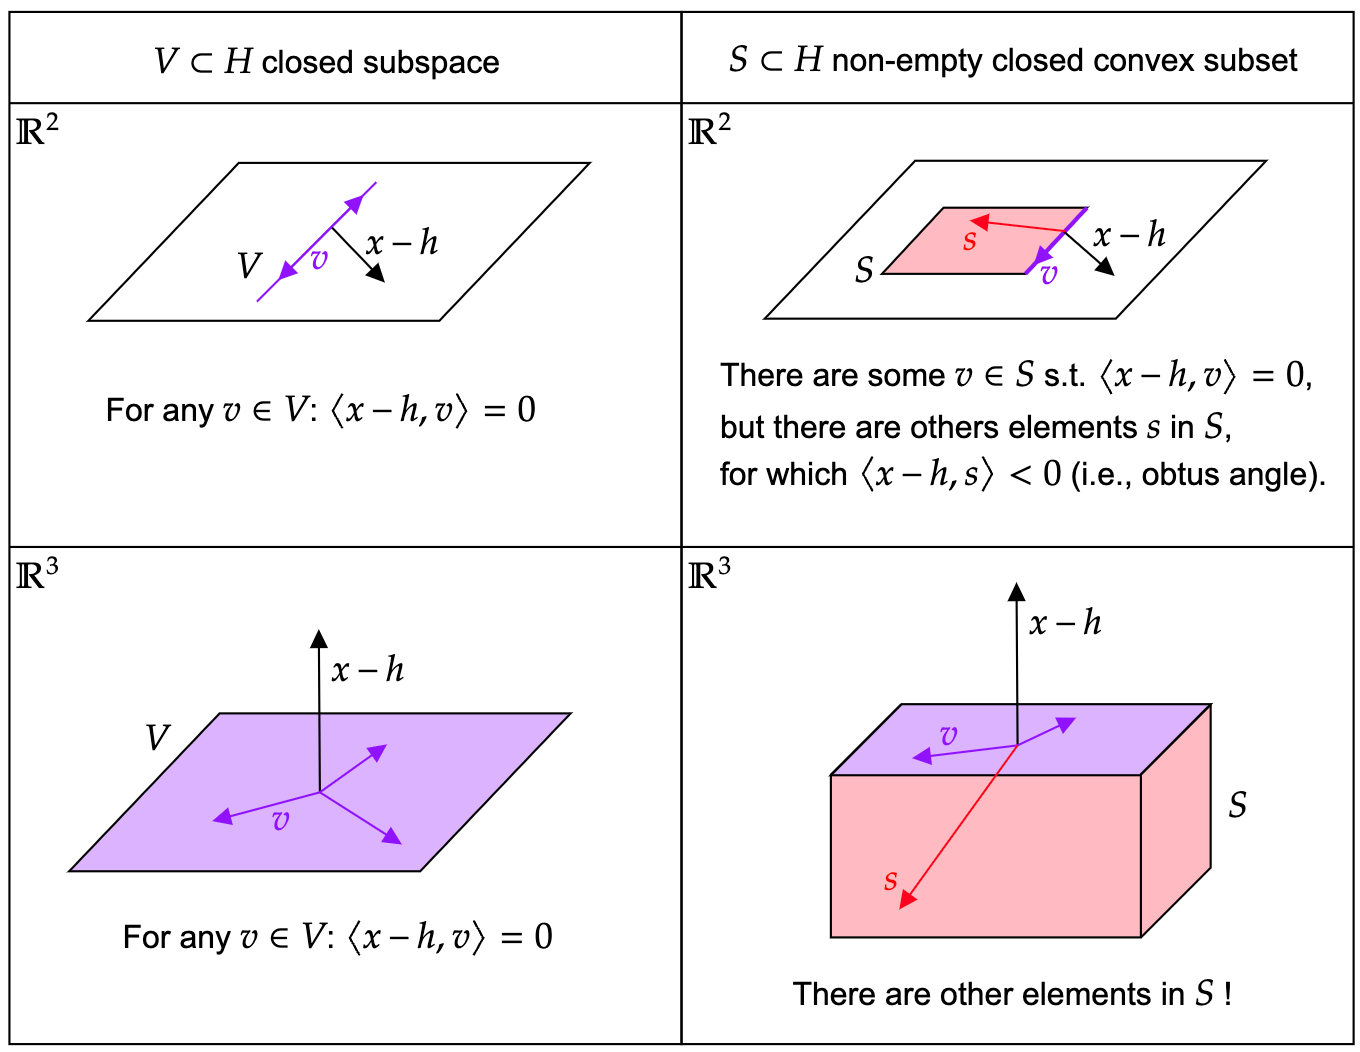
\includegraphics[width=14cm]{images/bonfa_1439.png}
\end{center}
\caption{}
\label{proj_fig3}
\end{figure}

\begin{proof}
We only show why there holds (\ref{proj_3}) in the particular case of subspace.

We start from (\ref{proj_2}):
\begin{equation*}
    \sca{x-h,v-h}\leq 0 \qquad \forall v\in V
\end{equation*}

Since $V$ is a subspace, $tv\in V$, so
\begin{equation*}
\sca{x-h,tv-h}\leq 0 \qquad \forall v\in V,\ \forall t\in\RR
\end{equation*}

We get
\begin{equation*}
    \sca{x-h,v}t-\sca{x-h,h}\leq 0 \qquad \forall v\in V,\ \forall t\in\RR
\end{equation*}

which implies $\sca{x-h,v}=0$ $\forall v\in V$ (line $y=mx-q\leq 0\ \forall x\in \RR$ implies $m=0$, i.e., when the line is horizontal).
\end{proof}

\begin{subtle}
In some sense, "you don't have only the segment, but the full line", i.e. every $h$ is the linear combination of $(1-t)v_1+tv_2$ with $t\in[-1,1]$, so you can redo the above proof just by relying on the proof of (c) in the general projection theorem proof: you find out the $\leq 0$ part by taking $t\in (0,1]$ (as we did) and the $\geq 0$ part by taking $t\in[-1,0)$, thus there holds the variational equality. 
\end{subtle}

\newpage

% direct sum

There exists another way to \emph{rephrase} the previous projection theorem, but before that we need some missing ingredient:

\begin{rem}
Let $V\subset \Hc$ subspace. Then:
\begin{enumerate}[(i)]
\item the followings are always closed:
\begin{itemize}
    \item $V$ if $\text{dim}(V)<\infty$
    \item $V^\perp$ $\big($ and this implies $\left( V^\perp \right)^\perp=\overline{V}\ \big)$
    \item $\text{ker}(L)$ if $L\in\rsf{L}(H,Y)$
\end{itemize}

\item the followings are never closed:
\begin{itemize}
    \item $V\subsetneqq \Hc$ dense
\end{itemize}

\item the followings aren't closed or open in general:
\begin{itemize}
    \item $R(L)$
\end{itemize}
\end{enumerate}
\end{rem}

\begin{defn}
Given $V,W\subset \Hc$ subspaces s.t. $V\cap W=\{ 0\}$. Then, the \textbf{direct sum} or \textbf{orthogonal sum} is
\begin{equation*}
V\oplus W = \left\{v+w\,:\,v\in V,\ w\in W \right\}
\end{equation*}
\end{defn}

\begin{es}
Prove that:
\begin{equation*}
\forall z \in V\oplus W \qquad \exists!\,v,w\quad\text{s.t.}\quad z=v+w
\end{equation*}
\end{es}

\begin{rem}
If $V$ is a subspace, then $V\cap V^\perp=\{0\}$.
\end{rem}

Here we come to the heart of the matter:

\begin{thm}
$\Hc$ Hilbert, $V$ closed subspace. Then:
\begin{equation*}
\qquad \qquad \Hc=V\oplus V^\perp \qquad \qquad (i)
\end{equation*}
More precisely:
\begin{enumerate}
\item[($ii$)] $\forall x\in \Hc$, $\ x=P_Vx+P_{V^\perp}x$ (unique decomposition)
\item[($iii$)] $x\in V\ \Leftrightarrow\ x=P_Vx\ $ and $\ x\in V^\perp\ \Leftrightarrow\ x=P_{V^\perp}x$
\item[($iv$)] $\norm{x}^2=\norm{P_Vx}^2+\norm{P_{V^\perp}x}^2$ ($\infty$-dim Pitagora theorem)
\item[($v$)] $P_V, P_{V^\perp} \in \rsf{L}(\Hc)$ and their norm is 1, i.e., they are linear and continuous operators which do not increase distance: $\norm{P_Vx_1-P_Vx_2}\leq\norm{x_1-x_2}$ $\ \forall x_1,x_2\in \Hc$.
\end{enumerate}
\end{thm}

\begin{proof}[just (\ref{proj_3})$\,\Rightarrow(ii)$, the others are simple implications]$\\$
First of all, we observe that the direct sum $V\oplus V^\perp$ is well-defined (see the above remark). Secondly, $P_Vx$ and $P_{V^\perp}x$ are well-defined thanks to the projection theorem for closed subspaces.

Now we can start. We have to prove that $P_{V^\perp}x=x-P_{V}x$. Since there holds (\ref{proj_3}), we know that
\begin{equation*}
\sca{x-P_{V^\perp}x,w}=0\qquad\forall w\in V^\perp
\end{equation*}

But you pay attention that also
\begin{equation*}
\sca{x-\left( x-P_Vx \right),w}=\langle \underbrace{P_Vx}_{\in V},\underbrace{w}_{\in V^\perp} \rangle=0 \qquad\forall w\in V^\perp
\end{equation*}

Hence $P_{V^\perp}x=x-P_{V}x$ (because the projection on $V^\perp$ has to be unique by (\ref{proj_1})).
\end{proof}

% section projections_onto_a_closed_convex_set (end)

\section{The Dual Space of a Hilbert Space} % (fold)
\label{sec:the_dual_space_of_a_hilbert_space}

Let $\Hc$ Hilbert. For any vector $u\in\Hc$ you can easily build an element $L_u\in\Hc^*$ of the dual with the scalar product:
\begin{equation*}
\forall u\in \Hc\quad \leadsto\quad L_u\in \Hc^*\quad\text{s.t.}\quad L_u v =\sca{u,v}\quad\forall v\in\Hc
\end{equation*}

\begin{subtle}
One can write $L_uv$ with the notation $\sca{L_u,v}$ and truly understand the link between these two things.
\end{subtle}

Then, $L_u$ is linear and continuous, indeed:
\begin{equation}
\label{dual_norm_eq}
{\renewcommand*{\arraystretch}{2.5}
\begin{array}{lclcl}
& & \overset{\underset{(\text{CS})}{}}{\leq} \displaystyle\sup_{x\neq 0} \dfrac{\norm{u}\cdot\cancel{\norm{x}}}{\cancel{\norm{x}}}=\norm{u} & & \\
& \nearrow & & \searrow & \\
\norm{L_u}_*=\displaystyle\sup_{x\neq 0} \dfrac{\left|L_ux\right|}{\norm{x}}=\displaystyle\sup_{x\neq 0} \dfrac{\abs{\sca{u,x}}}{\norm{x}}  & & & & = \norm{u}\\
& \searrow & & \nearrow \\
& & \overset{\underset{\text{sup}}{}}{\geq} \dfrac{\abs{\sca{u,\widetilde{x}}}}{\norm{\widetilde{x}}}\quad\text{for some } \widetilde{x}\neq 0 & & \\
& & \overset{\underset{\widetilde{x}=u\neq 0}{}}{=} \dfrac{\abs{\sca{u,u}}}{\norm{u}}=\dfrac{\norm{u}^{\cancel{2}}}{\norm{u}}=\norm{u} & & 
\end{array}}\qquad\qquad
\end{equation}

We obtain that
\begin{align*}
i:\Hc &\to \Hc^* \\
& u\mapsto L_u
\end{align*}

is an isometric embedding, i.e.
\begin{equation*}
\text{"}\Hc\subset\Hc^*\text{"}\qquad\text{or}\qquad \Hc \hookrightarrow \Hc^*
\end{equation*}

As always, we want to check if it is an isometric isomorphism, i.e.
\begin{equation*}
\Hc\ \text{"}=\text{"}\ \Hc^*\qquad\text{or}\qquad\Hc\simeq H^*\,,
\end{equation*}
or if there exists elements in the dual which do not come from elements in $\Hc$.

\bigskip
\bigskip

The answer is provided by the following theorem.

\newpage

\subsection{Riesz Representation Theorem}

\begin{thm}[Riesz Representation Theorem for $\Hc^*$]$\\$
$\Hc$ Hilbert. Then:
\begin{equation*}
\forall L\in \Hc^*\qquad \exists!\,u\in\Hc\quad\text{s.t.}\quad Lv=\sca{u,v}\quad\forall v\in\Hc
\end{equation*}
(you can think $L=L_u$). Moreover $\norm{u}=\norm{L}_*.$
\end{thm}

\begin{proof}
Firstly, we have to prove the existence of $u\in\Hc$ such that $\sca{u,v}=Lv$.

If $Lv=0$ $\,\forall v\in\Hc$, i.e. $\text{ker}\,L=\Hc$, just take $u=0$ and then you have
\begin{equation*}
\sca{0,v}=0=Lv\qquad \forall v\in \Hc
\end{equation*}

Now we are in the non-trivial situation, i.e. $\exists z_0\in \Hc\setminus\text{ker}\,L$. Since $\text{ker}\,L$ is closed, you can apply the projection theoem and find
\begin{equation*}
z=\frac{P_{(\text{ker}\,L)^\perp}z_0}{\norm{_{(\text{ker}\,L)^\perp}z_0}} 
\end{equation*}
such that $z\in(\text{ker}\,L)^\perp$ and $\norm{z}=1$.

Then, take $v\in\Hc$ and $w=v-\dfrac{Lv}{Lz}\ z$ so that 
\begin{equation*}
Lw=L\left( v-\frac{Lv}{Lz}\ z \right) = 0\qquad\Longrightarrow\qquad  w\in\text{ker}\,L
\end{equation*}

Finally
\begin{align*}
0&\overset{\underset{w\perp z}{}}{=}\sca{w,z} = \sca{v-\frac{Lv}{Lz}\ z,z}= \\
&=\sca{v,z}-\frac{Lv}{Lz}\underbracket[0.2pt]{\sca{z,z}}_{=\norm{z}^2=1}=\sca{v,z}-\frac{Lv}{Lz}
\end{align*}
i.e. 
\begin{equation*}
Lv=Lz\,\sca{v,z}=\sca{(Lz)z,v}\qquad\forall v\in\Hc
\end{equation*}
thus $u=(Lz)z$.

Secondly, we want to prove uniqueness. Let's assume $\exists$ $u_1,u_2$, $u_1\neq u_2$, s.t.
\begin{equation*}
Lv=\sca{u_1,v}\quad\text{and}\quad Lv=\sca{u_2,v}\qquad\forall v\in\Hc
\end{equation*}

Subtract the two equations and you have
\begin{equation*}
\sca{u_1-u_2,v}=0\qquad \forall v\in\Hc
\end{equation*}

Since the previous relation holds $\forall v\in\Hc$, you can take $v=u_1-u_2$ and obtain
\begin{equation*}
\sca{u_1-u_2,u_1-u_2}=0\qquad\overset{\underset{\text{positivity of }\sca{\cdot,\cdot}}{}}{\leadsto}
\qquad u_1-u_2=0
\end{equation*}
which contradict the assumption. So $u$ is unique.

\begin{subtle}
This explains why working with Hilbert spaces is much easier, because it is easy to say that zero is the only element orthogonal of itself. In just normed spaces of course you can use Hanh-Banach (\emph{bounded linear functionals separate points}) to say that zero is the only element orthogonal to everything, but it is required the axiom of choice.
\end{subtle}

The continuosly dependence from data is already proved in (\ref{dual_norm_eq}).
\end{proof}

So: $i$ is an isometric isomorphism, and we can identify $\Hc$ and $\Hc^*$.

\begin{subtle}
In reflexive spaces, when we identified $X$ and $X^{**}$ (thanks to $\tau$), we did it in a \emph{canonical way}, i.e. the indentification is independent of everything. Here, the identification between $\Hc$ and $\Hc^*$ is non canonical. For example, if you have $V\subsetneqq \Hc$ which is Hilbert too and dense, then $\Hc^*\subsetneqq V^*$. So, if you identify $\Hc$ and $\Hc^*$ then you cannot identify $V$ and $V^*$ (you can do that kind of identification only once, so it is not independent i.e. not canonical).
\end{subtle}


\begin{coro}
$\Hc$ Hilbert $\Longrightarrow$ $\Hc$ reflexive.
\end{coro}

Thanks to this fact, and thanks to Banach-Alaoglu thm (v1), every bounded sequence in $\Hc$ admits a subsequence which weakly converges.

\begin{proof}[just an idea]$\\$
We apply Riesz thm and we get $\Hc\simeq\Hc^*$, but then we can apply another time Riesz thm and get $\Hc^*\simeq\Hc^{**}$, so one can find a linear, continuous, injective, isometric canonical map that is surjective too and this implies reflexivity ($\Hc\simeq\Hc^{**}$ iff $\Hc$ is reflexive).

Another way to prove this corollary is via convexity: by the parallelogram identity, any Hilbert space is uniformly convex thus (Millman-Pettis) reflexive.
\end{proof}

\begin{rem}
The Riesz representation theorem is an example of \emph{well-posedness} problems (exists a unique solution which continuosly depends from data):
\begin{equation*}
    \boxed{\text{given }L\in\Hc^*\qquad\text{find }u\in\Hc\ :\ \sca{u,v}=Lv\quad\forall v\in\Hc }
\end{equation*}
Indeed, Riesz tells that $\exists !$ sol and then, since $\norm{u}=\norm{L}_*$, there holds the following stability estimate:
\begin{equation*}
    \norm{u_1-u_2}=\norm{L_1-L_2}_*
\end{equation*}
\end{rem}

\bigskip
\bigskip

The last, but not least, consequence of Riesz theorem is related to strong and weak convergence.

\newpage

\subsection{Convergences in Hilbert spaces}

Let's do some recalls ($X$ Banach, $\Hc$ Hilbert):
\begin{enumerate}[(i)]
\item \emph{Strong convergence.}
\begin{equation*}
x_n\to x\ \text{ strongly in }X\qquad\Longleftrightarrow\qquad\norm{x_n-x}_X\to 0\ \text{ in }\RR\ (\text{as }n\to+\infty)
\end{equation*}

\item \emph{Weak convergence.} 
\begin{equation*}
x_n\rightharpoonup x\ \text{ weakly in }X\qquad\Longleftrightarrow\qquad Lx_n\to Lx\ \text{ in }\RR\ (\text{as }n\to+\infty)\quad\forall L\in X^*
\end{equation*}

\item \emph{Property (c) of weak convergence.}
\begin{equation*}
x_n\rightharpoonup x\ \text{ weakly in }X\qquad\Longrightarrow\qquad \norm{x}_X\leq \liminf_n\norm{x_n}_X
\end{equation*}

Namely, weak convergence implies lower weak semicontinuity of $\norm{\cdot}$.

\item \emph{Weak convergence in Hilbert spaces.} Since every $L\in\Hc^*$ is just a scalar product, we can rephrase the definition of weak convergence in Hilbert spaces:
\begin{equation*}
x_n\rightharpoonup x\ \text{ weakly in }\Hc\qquad\Longleftrightarrow\qquad \sca{u,x_n}\to \sca{u,x}\ \text{ in }\RR\ (\text{as }n\to+\infty)\quad\forall u\in \Hc
\end{equation*}

\end{enumerate}

Here there comes the important fact:
\begin{proposition}
$\Hc$ Hilbert, $\left\{ x_n \right\}_{n\in\NN}\subset \Hc$. If
\begin{equation*}
\begin{cases}
    (\circledast)\ x_n\rightharpoonup x\ \text{ weakly in }\Hc\\
    (\star)\ \,\norm{x_n}\to\norm{x}\ \text{ as }n\to+\infty
\end{cases}
\end{equation*}
then $x_n\to x$ strongly in $\Hc$, i.e. $\norm{x_n-x}\to 0$.
\end{proposition}

\begin{proof}\leavevmode
\begin{equation*}
0\leq\norm{x_n-x}^2=\sca{x_n-x,x_n-x}=\underbracket[0.2pt]{\norm{x_n}^2}_{\overset{\underset{(\star)}{}}{\to}\norm{x}^2}-\underbracket[0.2pt]{2\sca{x_n,x}}_{\overset{\underset{(\circledast)}{}}{\to}2\sca{x,x}=2\norm{x}^2}+\norm{x}^2\to 0
\end{equation*}
\end{proof}

\emph{Remark 1.} This is an example which shows that: weak convergence + \emph{something} $\Rightarrow$ strong convergence.

\emph{Remark 2.} Since property (c), then the condition ($\star$) is not really absurd. Namely, it is sufficient to have also the other side
\begin{equation*}
    \limsup_n \norm{x_n}_X\leq \norm{x}_X
\end{equation*}

So, the \emph{something} we need to add to weak convergence in order to get strong convergence is precisely the previous inequality. Indeed, in the \emph{Functional Analysis, Sobolev Spaces and PDEs (Brezis)} book there is the following
\begin{proposition}
$X$ uniformly convex, $x_n\rightharpoonup x$ weakly in $X$ and $\limsup_n \norm{x_n}_X\leq \norm{x}_X$. Then $x_n\to x$ strongly in $X$.
\end{proposition}

% section the_dual_space_of_a_hilbert_space (end)

\newpage

\section{Orthonormal Basis} % (fold)
\label{sec:orthonormal_basis}

Let $\Hc$ Hilbert.

\begin{defn}
A sequence $\left\{ e_n \right\}_{n\in\NN}\subset\Hc$ is an \textbf{orthonormal basis} for $\Hc$ if
\begin{equation*}
    \norm{e_n}=1\quad\forall n\qquad\text{and}\qquad \sca{e_n,e_m}=0\quad\forall n\neq m
\end{equation*}
or
\begin{equation*}
\left\{ \text{all finite linear combination} \right\}=\text{span}\left( \left\{ e_n \right\}_n \right)\quad\text{is dense in }\Hc, \qquad\text{i.e. }\Hc=\overline{\text{span}\left( \left\{ e_n \right\}_n \right)}
\end{equation*}

\end{defn}

\begin{thm}
Every separable Hilbert space $\Hc$ has an orthonormal basis.
\end{thm}

\emph{Example.} $\Hc=\ell^2$ has $\left\{ e_n \right\}_n$ s.t.
\begin{equation*}
e_n=\left( e_n^{(1)}, e_n^{(2)},\dots \right) \quad\text{where}\quad e_n^{(k)}=\delta_{kn}=\begin{cases}
    1, &\text{ if }k=n\\
    0, &\text{ otherwise}
\end{cases}
\end{equation*}

\emph{Example.} $\Hc=L^2(-\pi,\pi)$ has
\begin{equation*}
\Bdu=\left\{ \frac{1}{\sqrt{2\pi}}, \frac{\sin nx}{\sqrt{\pi}} , \frac{\cos nx}{\sqrt{\pi}}, \ n=1,2,3,\dots  \right\}
\end{equation*}

\begin{thm}
Let $\left\{ e_n \right\}_n$ be an othonormal basis. Then, $\forall x\in \Hc$ you can write $x$ as a \textbf{generalized Fourier series}
\begin{equation*}
    x=\sum_{k=1}^\infty \sca{x,e_k}e_k
\end{equation*}
where $\sca{x,e_k}e_k$ is just $P_{\text{span}\{e_n\}}x$ and $\sca{x,e_k}$ are called \textbf{generalized Fuorier coefficients}. 

Moreover, there holds the \textbf{Parseval-Bessel identity} ($\infty$-dim Pitagora thm)
\begin{equation*}
    \norm{x}^2=\sum_{k=1}^\infty \abs{\sca{x,e_k}}^2
\end{equation*}
\end{thm}

\emph{Remark.} $\Hc$ separable, then 
\begin{align*}
    H&\simeq\ \ell^2 \\
    x&\leftrightarrow \left\{ \sca{x,e_k} \right\}_{k\in\NN}
\end{align*}

Here we notice the first example where there holds weak convergence but not strong convergence:
\begin{proposition}
$\Hc$ separable, $\left\{ e_n \right\}_n$ othonormal basis. Then $e_n\rightharpoonup 0$ weakly in $\Hc$, but not strongly.
\end{proposition}

\begin{proof}
$\forall n$, $\norm{e_n}=1\not\to0$, so $e_n\not\to 0$ strongly. On the other hand, $\forall x\in\Hc$
\begin{equation*}
\norm{x}^2=\sum_{n\in\NN}\abs{\sca{x,e_n}}^2
\end{equation*}
and since the series converges, its terms have to go necessarily to zero, i.e. $\sca{x,e_n}\to 0$, and this implies weak convergence (just by definition on Hilbert spaces).
\end{proof}

% section orthonormal_basis (end)

% ========================
% Poi da commentare
\setcounter{chapter}{14}
% ========================